In questo capitolo verrà affrontato il processo di \textbf{riconoscimento delle stanze} a partire dalle \textbf{mappa SLAM} generata attraverso i sensori LIDAR del robot. In particolare, verrà presentato il processo di individuazione proposto da \cite{mora}, le modifiche adottate e la console per poter visualizzare e modificare i risultati ottenuti.\\\\
I risultati ottenuti da questo processo verranno utilizzati per la generazione del grafo delle stanze nella mappa semantica.

\begin{figure}[H]
  \centering
  \includegraphics[width=\textwidth]{room_recognition/general_data_flow.png}
  \caption{Schema dei funzionamento per il riconoscimento delle stanze e il salvataggio del grafo delle stanze}
\end{figure}

\section{Grid maps}
Le Grid Maps sono \textbf{rappresentazioni spaziali dell'ambiente} che utilizzano una griglia per suddividere lo spazio in celle o pixel. In questo caso, sono utilizzate per rappresentare le grid map di occupazione, ovvero mappe in cui ogni cella può assumere uno dei seguenti valori:
\begin{itemize}
  \item Nero: se la cella è occupata. Tipicamente viene utilizzato per rappresentare le pareti o gli ostacoli presenti nell'ambiente;
  \item Bianco: se la cella è libera. Tipicamente viene utilizzato per rappresentare lo spazio libero, quello percorribile dal robot;
  \item Grigio: se la cella è sconosciuta. Tipicamente viene utilizzato per rappresentare le celle di cui non si ha informazione.
\end{itemize}
Questa tipologia di mappe è utilizzata per la navigazione dei robot autonomi, in quanto permette di \textbf{localizzarsi e mappare l'ambiente circostante simultaneamente} (SLAM).\\\\
Nel nostro caso, le grid map di occupazione vengono \textbf{generate dal modulo di navigazione} del robot e la loro immagine, in formato pgm, viene \textbf{utilizzata per il riconoscimento delle stanze}. In particolare, quando il modulo di navigazione effettua una richiesta http \apiurl{POST /navigation} al servizio di API per la creazione di una nuova mappa in contemporanea viene eseguito il job di Room Segmentation.

\begin{figure}[H]
  \centering
  \includegraphics[width=0.4\textwidth]{room_recognition/grid_map.png}
  \caption{Esempio di occupancy grid map utilizzata dal modulo di navigazione del robot}
\end{figure}

\section{Riconoscimento delle Stanze}
In questa sezione verrà presentato il processo di riconoscimento delle stanze proposto da \cite{mora} e basato sull'\textbf{algoritmo originale di Voronoi} \cite{thrun}.

\subsection{Segmentazione basata su Voronoi}
Il task del riconoscimento delle stanze è stato affrontato molto spesso nella letteratura. Ci sono infatti innumerevoli approcci per affrontare questo problema \cite{bormann}. Uno dei metodi più utilizzati è quello basato sull'algoritmo di Voronoi. Nel contesto di questa tesi, l'algoritmo di Voronoi \cite{thrun} è molto utile poichè genera anche un \textbf{grafo topologico} dove ogni nodo rappresenta una regione individuata e ogni arco rappresenta la connessione tra due di queste regioni. Questo è molto utile come base di partenza per la generazione del \textbf{grafo delle stanze}.\\\\
L'obiettivo dell'algoritmo di Voronoi è quello di decomporre le grid maps in un piccolo insieme di regioni separate da passaggi stretti e le porte, rappresentate da linee critiche. Questo processo è composto da tre fasi principali:
\begin{itemize}
  \item Binarizzazione: trasformazione della occupancy grid map in una mappa binaria; le celle con valori superiori della soglia sono considerate spazio libero $C$. Tutte le altre come spazio occupato $\bar{C}$;
  \item Costruzione del Diagramma di Voronoi: Per ogni punto $p = <x, y> \in C$, esistono uno o più punti vicini $s \in \bar{C}$. Questi punti vengono chiamati \textit{punti base} di $<x, y>$ e la distanza tra $<x, y>$ e i suoi punti base come \textit{clearance} di $<x, y>$\\
        \begin{equation}
          \text{punti base} = \{s \mid s \in \bar{C}, \text{dist}(p, s) = \min_{s \in \bar{C}} \{\text{dist}(p,s)\}\}
        \end{equation}
        \begin{equation}
          \text{clearance}(p) = \min_{s \in \text{punti base}} \{\text{dist}(p,s)\}
        \end{equation}
        Il diagramma di Voronoi è l'insieme dei punti $p \in C$ che hanno almeno due punti base equidistanti diversi;
  \item Identificazione dei punti critici: punti $p \in C$ che minimizzano la \textit{clearance} localmente. In teoria corrispondono ai passaggi stretti e alle porte.\\\\
        L'approccio proposto da \cite{mora}, e utilizzato in questo lavoro, si basa sugli stessi concetti base dell'algoritmo di Voronoi, ma con alcune modifiche per migliorare la qualità dei risultati. In particolare, analizza sia lo \textbf{spazio libero}, ricercando i punti critici che chiama \textit{intersection points}, sia lo \textbf{spazio occupato}, ricercando gli \textit{endpoints} di ogni ramo del diagramma di Voronoi dello spazio occupato. Questi dati sono successivamente utilizzati per individuare le linee critiche e separare quindi le regioni.
\end{itemize}
\begin{figure}[H]
  \centering
  \begin{subfigure}[t]{0.45\textwidth}
    \centering
    \includegraphics*[width=\textwidth]{room_recognition/voronoi_examples/voronoi_example_map.png}
    \caption{Grid Map d'esempio}
  \end{subfigure}
  \hfill
  \begin{subfigure}[t]{0.45\textwidth}
    \centering
    \includegraphics[width=\textwidth]{room_recognition/voronoi_examples/voronoi_example_skeleton.png}
    \caption{Diagramma di Voronoi}
  \end{subfigure}\\
  \begin{subfigure}[t]{0.45\textwidth}
    \centering
    \includegraphics*[width=\textwidth]{room_recognition/voronoi_examples/voronoi_example_critical_points.png}
    \caption{Punti Critici}
  \end{subfigure}
  \hfill
  \begin{subfigure}[t]{0.45\textwidth}
    \centering
    \includegraphics[width=\textwidth]{room_recognition/voronoi_examples/voronoi_example_critical_lines.png}
    \caption{Linee Critiche}
  \end{subfigure}
  %\end{figure}
  %\begin{figure}[H]
  \begin{subfigure}[t]{0.45\textwidth}
    \centering
    \includegraphics*[width=\textwidth]{room_recognition/voronoi_examples/voronoi_example_map_regions.png}
    \caption{Regioni}
  \end{subfigure}
  \hfill
  \begin{subfigure}[t]{0.45\textwidth}
    \centering

    \begin{tikzpicture}[
      >={Stealth[round]},  % Arrow tip
      auto,
      thick  % Line thickness
      ]

      % Definire le coordinate dei centri delle regioni (questi sono esempi, dovrai aggiustarli secondo la tua immagine)
      \node (A) [circle, draw, scale=0.8, fill=red!20] at (4.5,4.3) {R1}; % Regione rossa
      \node (B) [circle, draw, scale=0.8, fill=blue!20] at (1.7,2.8) {R2}; % Regione blu
      \node (C) [circle, draw, scale=0.8, fill=green!20] at (5.8,2.2) {R3}; % Regione verde
      \node (D) [circle, draw, scale=0.8, fill=yellow!20] at (4,0.8) {R4}; % Regione gialla

      \node(O) at (1.7,0){};

      \draw[<->] (A) -- (B);
      \draw[<->] (A) -- (C);
      \draw[<->] (B) -- (D);
      \draw[<->] (C) -- (D);

    \end{tikzpicture}
    \caption{Grafo topologico}
  \end{subfigure}
  \caption{Esempio di riconoscimento delle stanze tramite l'algoritmo di Voronoi originale \cite{thrun}}
\end{figure}

\subsection{Preprocessing}
In questa fase, l'immagine della mappa viene binarizzata e si cerca di limitare il rapporto Signal-to-Noise (SNR) per migliorare la qualità dei risultati.
\subsubsection{Binarizzazione}
L'immagine della mappa viene binarizzata due volte, una volta per la generazione della maschera dello spazio libero e una volta per la generazione della maschera per lo spazio occupato. Questo processo è necessario per poter analizzare separatamente i due spazi.

\begin{figure}[H]
  \begin{subfigure}[t]{0.45\textwidth}
    \centering
    \includegraphics[width=\textwidth]{room_recognition/mora/bin_free_space.png}
    \caption{Immagine binaria dello spazio libero}
  \end{subfigure}
  \hfill
  \begin{subfigure}[t]{0.45\textwidth}
    \centering
    \includegraphics[width=\textwidth]{room_recognition/mora/bin_occupied_space.png}
    \caption{Immagine binaria dello spazio occupato}
  \end{subfigure}
\end{figure}

\subsubsection{Morfologia matematica}
In questa fase vengono applicate delle operazioni di morfologia matematica per ridurre il rumore. In base alla tipologia di spazio analizzato, vengono applicate operazioni diverse, anche per accentuare elementi diversi.

\paragraph{Spazio libero}
Viene applicato un processo di erosione con un elemento strutturante elissoidale di dimensione 5x5. Successivamente si applica un filtro mediano 5x5 per rimuove il rumore sale e pepe e per smussare gli angoli.

\paragraph{Spazio occupato}
Viene applicato un processo di dilatazione con un elemento strutturante quadrato di dimensione 5x5.

\begin{figure}[H]
  \begin{subfigure}[t]{0.45\textwidth}
    \centering
    \includegraphics[width=\textwidth]{room_recognition/mora/preprocessed_free_space.png}
    \caption{Immagine binaria dello spazio libero dopo il preprocessing}
  \end{subfigure}
  \hfill
  \begin{subfigure}[t]{0.45\textwidth}
    \centering
    \includegraphics[width=\textwidth]{room_recognition/mora/preprocessed_occupied_space.png}
    \caption{Immagine binaria dello spazio occupato dopo il preprocessing}
  \end{subfigure}
\end{figure}
\subsection{Analisi dello spazio libero}
L'obiettivo di questa fase è quello di \textbf{individuare i punti critici} e le linee critiche che giacciono in corrispondenza dei passaggi stretti.
\subsubsection{Diagramma di Voronoi}
Si procede con il determinare il diagramma di Voronoi dello spazio libero. Nel paper originale viene utilizzato lo scheletro della mappa binaria come approssimazione di Voronoi. In questo lavoro, viene invece utilizzata la \textbf{trasformata asse mediano} poichè si è empiricamente notato che fornisce risultati migliori.

\subsubsection{Branching}
Si individuano nel diagramma di Voronoi i punti di branching ovvero i punti dove il diagramma si biforca. Per individuarli si utilizza la trasformata HIT or MISS con i kernels 3x3 seguenti:
\begin{figure}[H]
  \centering
  \begin{subfigure}[t]{\textwidth}
    \centering
    \includegraphics[width=0.9\textwidth]{room_recognition/mora/branching_points_kernels_1.png}
    \caption{Kernels per i branch a T}
  \end{subfigure}\\
  \begin{subfigure}[t]{\textwidth}
    \centering
    \includegraphics[width=0.9\textwidth]{room_recognition/mora/branching_points_kernels_2.png}
    \caption{Kernels per i branch a Y}
  \end{subfigure}\\
  \caption{Kernels per l'individuazione dei punti di branch. In nero i valori -1, in grigio i valori 0 e in bianco i valori 1 dei kernels}
\end{figure}
\noindent
Successivamente si procede con la rimozione dei punti di branch dal diagramma di Voronoi e si effettua il {labeling delle componenti connesse}, in modo da poter individuare ogni ramo del diagramma. I rami il cui numero di pixels è inferiore a dieci pixels vengono eliminati.
\begin{figure}[H]
  \centering

  \begin{subfigure}[t]{.45\textwidth}
    \centering
    \includegraphics[width=0.98\textwidth]{room_recognition/mora/free_space_voronoi_diagram.png}
    \caption{Diagramma di Voronoi approssimato}
  \end{subfigure}
  \begin{subfigure}[t]{.45\textwidth}
    \centering
    \includegraphics[width=0.98\textwidth]{room_recognition/mora/free_space_diagram_endpoints.png}
    \caption{Punti di branch del diagramma di Voronoi}
  \end{subfigure}\\
  \begin{subfigure}[t]{.45\textwidth}
    \centering
    \includegraphics[width=0.98\textwidth]{room_recognition/mora/free_space_diagram_no_branch_points.png}
    \caption{Differenza tra il diagramma di Voronoi e i punti di branch}
  \end{subfigure}
  \begin{subfigure}[t]{.45\textwidth}
    \centering
    \includegraphics[width=0.98\textwidth]{room_recognition/mora/free_space_diagram_branches_labeling.png}
    \caption{Labeling delle componenti connesse dell'immagine {(c)}}
  \end{subfigure}
  \caption{Processo di individuazione dei punti di branch}
\end{figure}

\subsubsection{Ricerca dei segmenti}
Per ogni ramo del diagramma di Voronoi si procede con la ricerca dei segmenti. \\
Un segmento è definito come l'insieme di punti del branch che hanno una clearance nell'intorno di due pixels rispetto alla clearance minima del branch.
\begin{equation}
  \text{segmento} = \{p \mid | \text{clearance}(p) - \text{clearance}_{\text{min}} | \leq 2\}
\end{equation}
A supporto dell'individuazione dei segmenti, si calcola la \textbf{trasformata distanza} che assegna a ogni pixel il valore della distanza minima da un pixel dello spazio occupato e si utilizza per calcolare la clearance di ogni punto del branch.\\Per ogni segmento si salva centroide e orientamento.
\begin{figure}[H]
  \centering
  \includegraphics[width=0.441\textwidth]{room_recognition/mora/free_space_distance_tr.png}
  \caption{Trasformata distanza dello spazio libero}
\end{figure}
\paragraph{Calcolo orientamento del segmento}
Si trovano gli endpoints $a$ e $b$ (attraverso la trasformata HIT or MISS con kernels che verranno approfonditi nella sezione successiva) e si calcola l'orientamento del segmento come l'angolo tra la retta passante per gli endpoints e l'asse x.\\
In particolare, se la retta passante per i due punti non è verticale, si calcola $m = \frac{y_a - y_b}{x_a-x_b}$, coefficiente angolare della retta e si calcola l'orientamento come $\theta = \arctan(m)$.
\begin{equation}
  \theta = \begin{cases}
    \arctan( \frac{y_a - y_b}{x_a-x_b}) & \text{se } x_a \neq x_b \\
    \frac{\pi}{2}                       & \text{altrimenti}
  \end{cases}
\end{equation}
È bene notare che il sistema di riferimento delle immagini è invertito rispetto a quello classico, con l'asse y che cresce verso il basso. Di conseguenza, la funzione $\arctan$ di $numpy$ restituisce i valori diversi da quelli che si aspetterebbe. \\
Per esempio, nella figura sottostante, numpy restituisce l'algolo $\alpha$ invece di $\beta$. Per ovviare a questo problema, l'angolo finale viene calcolato come $\theta = \pi - \alpha$.
\begin{figure}[H]
  \centering
  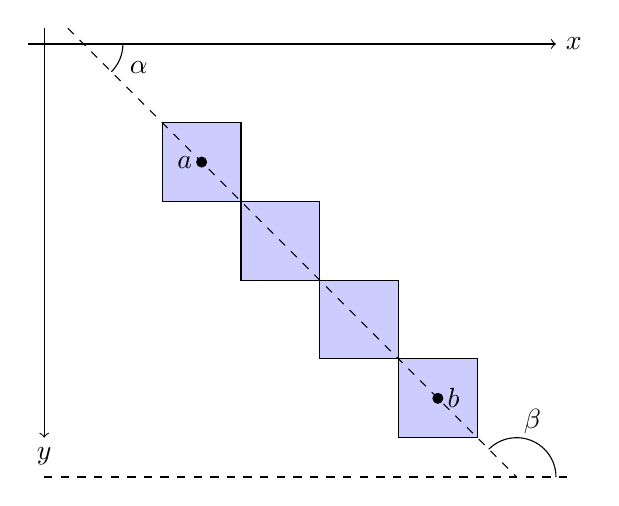
\begin{tikzpicture}
    % Draw x and y axes
    \draw[->] (0.3,0) -- (7,0) node[right] {$x$};
    \draw[->] (0.5,0.2) -- (0.5,-5) node[below] {$y$};

    % Draw the staircase
    \foreach \i in {1,...,4} {
        \draw[fill=blue!20] (\i+1,-\i) rectangle (\i+2,-\i-1);
      }

    % Draw the dashed line and the angles
    \draw[dashed] (0.8,0.2) -- (6.5,-5.5);
    \draw[dashed] (0.5,-5.5) -- (7.2,-5.5);

    \draw[-] (1.5,0) arc[start angle=0,end angle=-45,radius=0.5];
    \node at (1.7,-0.3) {$\alpha$};

    \draw[-] (7,-5.5) arc[start angle=0,end angle=135,radius=0.5];
    \node at (6.7,-4.8) {$\beta$};

    \coordinate (a) at (2.5, -1.5);
    \coordinate (b) at (5.5, -4.5);
    % Add labels
    \node at (a) [left] {$a$};
    \node at (b) [right] {$b$};

    \foreach \point in {a,b}
    \fill [black,opacity=1] (\point) circle (2pt);
  \end{tikzpicture}
  \caption {Calcolo dell'orientamento del segmento. I quadrati in blu rappresentano i pixel del segmento}
\end{figure}
\noindent
Inoltre, $\alpha$ è positivo in verso orario e negativo in verso antiorario. In quest'ultimo caso, l'angolo finale viene calcolato come $\theta = -\alpha$.
\begin{equation}
  \theta = \begin{cases}
    \pi - \alpha & \text{se } y_a < y_b \land x_a < x_b \\
    -\alpha      & \text{altrimenti}
  \end{cases}
\end{equation}
\subsubsection{Ricerca degli intersection points}
Un intersection point è definito come il punto nello spazio occupato più vicino al centroide di un segmento lungo la direzione perpendicolare all'orientamento del segmento.\\
A supporto dell'inviduazione degli intersection points, si utilizza la trasformata distanza per determinare di quanto scalare il vettore perpendicolare al segmento per trovare il punto più vicino nello spazio occupato. Gli intersection points vengono dunque calcolati come:
\begin{equation}
  ip_1 =
  \begin{bmatrix}
    x_{\text{centroid}} \\
    y_{\text{centroid}}
  \end{bmatrix} +
  \begin{bmatrix}
    \cos(\theta + \frac{\pi}{2}) \\
    \sin(\theta + \frac{\pi}{2})
  \end{bmatrix} \cdot \text{dist}(x_{\text{centroid}}, y_{\text{centroid}})\\
\end{equation}
\begin{equation}
  ip_2 =
  \begin{bmatrix}
    x_{\text{centroid}} \\
    y_{\text{centroid}}
  \end{bmatrix} +
  \begin{bmatrix}
    \cos(\theta - \frac{\pi}{2}) \\
    \sin(\theta - \frac{\pi}{2})
  \end{bmatrix} \cdot \text{dist}(x_{\text{centroid}}, y_{\text{centroid}})
\end{equation}
Per ogni segmento si determinano quindi gli intersection points i quali delimitano una possibile linea critica tra due regioni.

\begin{figure}[H]
  \centering
  \includegraphics[width=0.5\textwidth]{room_recognition/mora/segments_and_intersections_lines.png}
  \caption{Segmenti e intersection points. In rosso i segmenti, in verde le linee critiche delimitate dagli intersection points, in blu il diagramma di Voronoi}
\end{figure}
\subsection{Analisi dello spazio occupato}
L'obiettivo di questa fase è quello di individuare i cosidetti endpoints, ovvero i punti che delimitano i rami del diagramma di Voronoi dello spazio occupato. Questi punti sono utili per scremare dalle linee critiche quelle che non sono effettivamente delle porte, come verrà illustrato nella sezione successiva
\subsubsection{Diagramma di Voronoi}
Così come per lo spazio libero, anche per lo spazio occupato viene determinato il diagramma di Voronoi approssimato alla \textbf{trasformata asse mediano}. Si ottiene dunque una foresta di diagrammi di Voronoi,ognuno dei quali corrisponde a una zona occupata diversa. \\
I diagrammi con meno di 20 pixels vengono scartati, in modo da rimuovere i diagrammi relativi alle piccole zone che normalmente corrispondono a errori di mappattura dovuti al rumore.

\begin{figure}[H]
  \centering
  \begin{subfigure}[t]{0.45\textwidth}
    \centering
    \includegraphics[width=\textwidth]{room_recognition/mora/occupied_space_voronoi_diagram.png}
    \caption{Diagramma di Voronoi dello spazio occupato}
  \end{subfigure}
  \begin{subfigure}[t]{0.45\textwidth}
    \centering
    \includegraphics[width=\textwidth]{room_recognition/mora/occupied_space_diagram_branches_labeling.png}
    \caption{Labeling delle componenti connesse di (a)}
  \end{subfigure}
\end{figure}

\subsubsection{Ricerca degli endpoints}
I diagrammi di voronoi estratti dallo spazio occupato sono utili per la ricerca delle protuberanze presenti vicino alle porte. Queste protuberanze sono individuate come endpoints, localizzati attraverso l'utilizzo della trasformata HIT or MISS con i kernels 3x3 seguenti:
\begin{figure}[H]
  \centering
  \includegraphics[width=0.9\textwidth]{room_recognition/mora/endpoints_kernels.png}
  \caption{In nero i valori -1, in grigio i valori 0 e in bianco i valori 1 dei kernels}
\end{figure}
\begin{figure}[H]
  \centering
  \includegraphics[width=0.5\textwidth]{room_recognition/mora/occupied_space_diagram_endpoints.png}
  \caption{Diagramma di Voronoi dello spazio occupato con gli endpoints evidenziati in rosso}
\end{figure}
\subsection{Ricerca delle porte}
Le porte sono definite come passaggi stretti nello spazio libero dove vi è la presenza di protuberanze dello spazio occupato.\\
Utilizzando entrambe le tipologie di informazioni estrapolate negli step precedenti, è possibile individuare in modo abbastanza preciso le linee critiche che effettivamente dividono due stanze. \\\\
Il primo passo è quello di individuare, per ciascun intersection point dello spazio libero, l'endpoint dello spazio occupato più vicino. Unendo gli endpoint $ce1, ce2$ più vicini rispettivamente al primo e al secondo intersection point, si ottiene un'ulteriore linea $\overline{ce_1ce_2}$.\\

Infine, se:
\begin{itemize}
  \item $distance(ip_1, ce_1) \leq \frac{threshold}{2}$
  \item $distance(ip_2, ce_2) \leq \frac{threshold}{2}$
  \item $distance(ip_{centroid}, ce_{centroid}) \leq threshold$
  \item il segmento $\overline{ip_1ip_2}$ non interseca alcun diagramma di Voronoi dello spazio occupato
\end{itemize}
Allora questo rappresenta una door location valida.\\\\
Uno dei vantaggi di questa approccio è che la soglia \textit{threshold} non è fissa: viene infatti calcolata per ogni mappa come la media dei valori della trasformata distanza dello spazio occupato nei punti dove è presente il suo diagramma di Voronoi, moltiplicata per due. Rappresenta la larghezza media dei muri nella mappa analizzata.
\begin{figure}
  \centering
  \begin{subfigure}[t]{0.45\textwidth}
    \centering
    \includegraphics[width=\textwidth]{room_recognition/mora/segments_intersection_closest_endpoints.png}
    \caption{Segmenti, intersection points e endpoints. In giallo i segmenti che congiungono gli endpoints più vicini}
  \end{subfigure}
  \begin{subfigure}[t]{0.45\textwidth}
    \centering
    \includegraphics[width=\textwidth]{room_recognition/mora/segments_valid_doors.png}
    \caption{Segmenti, intersection points e endpoints che soddisfano le condizioni e quindi sono elegibili come porte}
  \end{subfigure}
\end{figure}
\subsection{Separazione delle stanze}
Si procede infine con la separazione delle stanze. Per ogni segmento in prossimità di una porta valida, si crea la maschera della linea critica che viene sottratta alla maschera dello spazio libero. Successivamente si esegue il labeling delle componenti connesse, e dopo aver filtrato le stanze con area inferiore a trenta pixels, si ottengono le stanze separate.
\begin{figure}[H]
  \centering
  \includegraphics[width=0.45\textwidth]{room_recognition/mora/rooms.png}
  \caption{Stanze separate}
\end{figure}
Come si può notare, ci sono delle incorrettezze. Tuttavia, queste possono essere corrette con l'ausilio dell'utente, come verrà illustrato nella sezione successiva.

\subsection{Generazione Grafo delle Stanze}
Il grafo delle stanze viene generato a partire dalle stanze separate e dai segmenti validi.\\\\
Viene creato un nodo per ogni stanza individuata. La \textbf{lista di segmenti} rappresentante il perimetro della stanza viene determinata approssimando il contorno della maschera della stanza con l'\textbf{algoritmo di Ramer–Douglas–Peucker} implementato in OpenCV.\\
Per ogni segmento valido, si controlla la label di appartenenza degli estremi del segmento che teoricamente giacciono in due stanze diverse, e si crea un arco tra i due nodi delle stanze corrispondenti. \\
Infine se eliminano i nodi che non sono connessi a nessun arco, rimuovendo così le stanze isolate che per definizione non dovrebbero esistere.
\begin{figure}[H]
  \centering
  \begin{tikzpicture}[
    >={Stealth[round]},  % Arrow tip
    auto,
    thick  % Line thickness
    ]
    \node (a) [circle, draw, scale=0.8, fill=teal!20] {Stanza 1};
    \node (fake) [above=of a]{};
    \node (b) [circle, draw, scale=0.8, fill=green!20, left=of fake] {Stanza 2};
    \node (c) [circle, draw, scale=0.8, fill=yellow!20, right=of fake] {Stanza 3};
    \node (d) [circle, draw, scale=0.8, fill=orange!20, below=of c] {Stanza 4};
    \node (e) [circle, draw, scale=0.8, fill=magenta!20, below=of b] {Stanza 5};
    \node (f) [circle, draw, scale=0.8, fill=red!20, left=of e] {Stanza 6};
    \node (g) [circle, draw, scale=0.8, fill=blue!20, below=e] {Stanza 7};
    \node (h) [circle, draw, scale=0.8, fill=purple!20, below=of d] {Stanza 8};

    \draw [<->] (a) -- (b);
    \draw [<->] (a) -- (c);
    \draw [<->] (a) -- (d);
    \draw [<->] (a) -- (e);
    \draw [<->] (f) -- (e);
    \draw [<->] (a) -- (g);
    \draw [<->] (a) -- (h);
  \end{tikzpicture}
  \caption{Grafo delle stanze generato a partire dalle stanze separate}
\end{figure}
\section{Visualizzazione e Modifica delle Stanze}
Affinchè l'utente possa visualizzare i risultati del riconoscimento e modificare la divisione in stanze aggiugendone di nuove, eliminandone o modificandone di esistenti, è stato sviluppato un tool grafico all'interno della webapp già esistente per la gestione di Robee, la cosidetta \textit{console}. Il funzionamento della console esula dagli obiettivi di questa tesi, tuttavia è importante illustrare come è stata integrata la funzionalità di visualizzazione e modifica delle stanze all'interno di essa.
\subsection{Layers e modelli}
A supporto di tale feature sono stati creati dei modelli per rappresentare un generico \textit{layer} della mappa, anche in vista di futuri sviluppi, composto da una lista di \textit{layer area} che rappresentano delle zone all'interno della mappa. La classe \textit{layer area outline} rappresenta il contorno di una layer area.
\begin{figure}[H]
  \centering
  \scalebox{0.84}{
    \begin{tikzpicture}
      \umlclass[x=5, y=0]{Layer}{
        + enabled : bool \\
        + filled : bool \\
        + name : string \\
        + areas : List[LayerArea]
      }{}

      \umlclass[x=10, y=0]{LayerArea}{
        + id : string \\
        + label : string \\
        + outline: LayerAreaOutline \\
        + color : string
      }{}

      \umlclass[x=15, y=0]{LayerAreaOutline}{
        + points : List[Position]
      }{}

    \end{tikzpicture}
  }
  \caption{Classi per la gestione dei layer}
\end{figure}
\noindent
Per la gestione delle stanze, ogni layer area rappresenta il poligono della stanza.

\subsection{Schema di funzionamento}
\begin{figure}[H]
  \centering
  \includegraphics[width=0.95\textwidth]{room_recognition/console_data_flow.png}
  \caption{Schema di funzionamento per la visualizzazione e modifica delle stanze}
\end{figure}
Console Service è la webapp per la gestione di Robee, sviluppata con Python, Tornado, Turbo e Stimulus JS e che sfrutta il pattern MVC.\\\\
Quando un utente visita la pagina per la visualizzazione di una mappa, il server scarica l'immagine della mappa e costruisce l'html dal template iniettando i dati necessari e restituendo la pagina all'utente.\\ Successivamente, quando questo seleziona la visualizzazione del layer delle stanze dal menu a tendina, il client effettua una chiamata http \apiurl{GET /rooms} al server che esegue una query al db, costruisce i modelli e li restituisce al client che renderizza i poligoni delle stanze in un canvas sovrapposto all'immagine della mappa.\\
\subsection{Features}
\begin{figure}[H]
  \centering
  \includegraphics[width=\textwidth]{room_recognition/console/room_home.png}
  \caption{Pagina di visualizzazione delle stanze}
\end{figure}

\protect
\subsubsection{Taglio di una stanza}
Selezionando la modalità \textit{cut} e cliccando su due punti del contorno del poligono di una stanza, la si taglia, creandone due nuove.
\begin{figure}[H]
  \begin{subfigure}[t]{0.50\textwidth}
    \centering
    \includegraphics[width=\textwidth]{room_recognition/console/room_cut_before.png}
  \end{subfigure}
  \begin{subfigure}[t]{0.50\textwidth}
    \centering
    \includegraphics[width=\textwidth]{room_recognition/console/room_cut_after.png}
  \end{subfigure}
\end{figure}

\protect
\subsubsection{Nuovo punto nel poligono di una stanza}
Selezionando la modalità \textit{add}, dopo aver selezionato un punto del poligono, con un doppio click è possibile creare un nuovo punto successivo a quello selezionato precedentemente.
\begin{figure}[H]
  \begin{subfigure}[t]{0.50\textwidth}
    \centering
    \includegraphics[width=\textwidth]{room_recognition/console/room_add_before.png}
  \end{subfigure}
  \begin{subfigure}[t]{0.50\textwidth}
    \centering
    \includegraphics[width=\textwidth]{room_recognition/console/room_add_after.png}
  \end{subfigure}
\end{figure}

\protect
\subsubsection{Eliminazione di una stanza}
Selezionando la modalità \textit{delete}, è possibile eliminare una stanza cliccando su una qualsiasi parte di essa.
\begin{figure}[H]
  \begin{subfigure}[t]{0.50\textwidth}
    \centering
    \includegraphics[width=\textwidth]{room_recognition/console/room_delete_before.png}
  \end{subfigure}
  \begin{subfigure}[t]{0.50\textwidth}
    \centering
    \includegraphics[width=\textwidth]{room_recognition/console/room_delete_after.png}
  \end{subfigure}
\end{figure}

\protect
\subsubsection{Creazione di una nuova stanza}
Selezionando la modalità \textit{add}, senza aver selezionato un qualsiasi punto di una stanza è possibile creare una nuova stanza facendo doppio click su un qualsiasi spazio vuoto della mappa. Non sono ammessi sovrapposizioni.
\begin{figure}[H]
  \begin{subfigure}[t]{0.50\textwidth}
    \centering
    \includegraphics[width=\textwidth]{room_recognition/console/room_new_before.png}
  \end{subfigure}
  \begin{subfigure}[t]{0.50\textwidth}
    \centering
    \includegraphics[width=\textwidth]{room_recognition/console/room_new_after.png}
  \end{subfigure}
\end{figure}

\protect
\subsubsection{Spostamento di un punto del poligono di una stanza}
Selezionando la modalità \textit{move}, è possibile spostare un punto del poligono della stanza cliccando su di esso e trascinandolo.
\begin{figure}[H]
  \begin{subfigure}[t]{0.50\textwidth}
    \centering
    \includegraphics[width=\textwidth]{room_recognition/console/room_move_before.png}
  \end{subfigure}
  \begin{subfigure}[t]{0.50\textwidth}
    \centering
    \includegraphics[width=\textwidth]{room_recognition/console/room_move_after.png}
  \end{subfigure}
\end{figure}

\section{Conclusioni}
In questo capitolo è stato affrontanto il processo di \textbf{riconoscimento delle stanze} a partire dalle mappe SLAM generate dai sensori LIDAR del robot. In particolare, è stato presentato il processo di individuazione proposto da \cite{mora} e basato su \textbf{Voronoi} \cite{thrun} che, prima dell'implementazione sembrava molto preciso ed efficace ma che tuttavia così non si è rivelato. Per questo motivo è stato sviluppato uno strumento che oltre alla classica visualizzazione dei risultati consente anche di \textbf{modificare la disposizione delle stanze}, come i classici strumenti di annotazione delle immagini. Le \textbf{annotazioni} delle stanze corrette, in futuro, potranno essere utilizzati come dati di \textbf{training} di un modello di machine learning apposito.\\Inoltre si potrebbe pensare di sperimentare tecniche di riduzione del rumore più avanzate, come proposto da \cite{rose}